\begin{figure}[!h] 
	\vspace{-10pt}
	\centering
	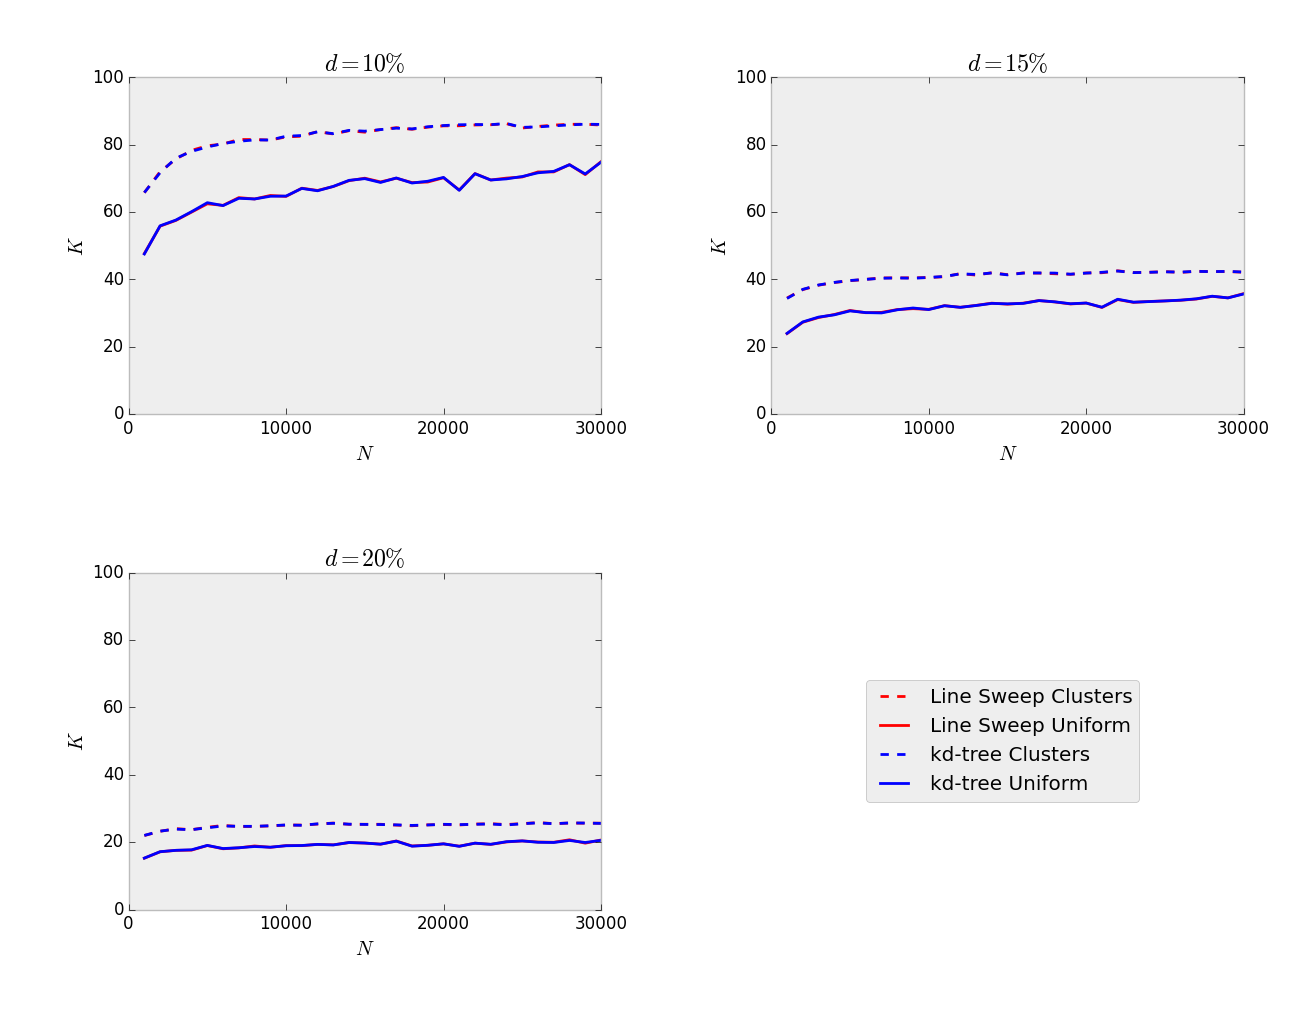
\includegraphics[width=\linewidth]{Pictures/ls_kd_k} 
	\caption[Number $k$ of points selected for Line Sweep and $k$-d Tree range search.]{Number $k$ of points selected for both proximity graph algorithms on uniform and clustered inputs for different values of $d$. Note that the lines overlap, since both algorithms are expected to output the same set most of the time.}
	\label{fig:ls_kd_k} 
\end{figure}